\documentclass[tikz,border=10pt]{standalone}
\usepackage{amsmath,amssymb}
\usetikzlibrary{arrows.meta,positioning,calc,fit,decorations.pathreplacing,shadows.blur}

\begin{document}
	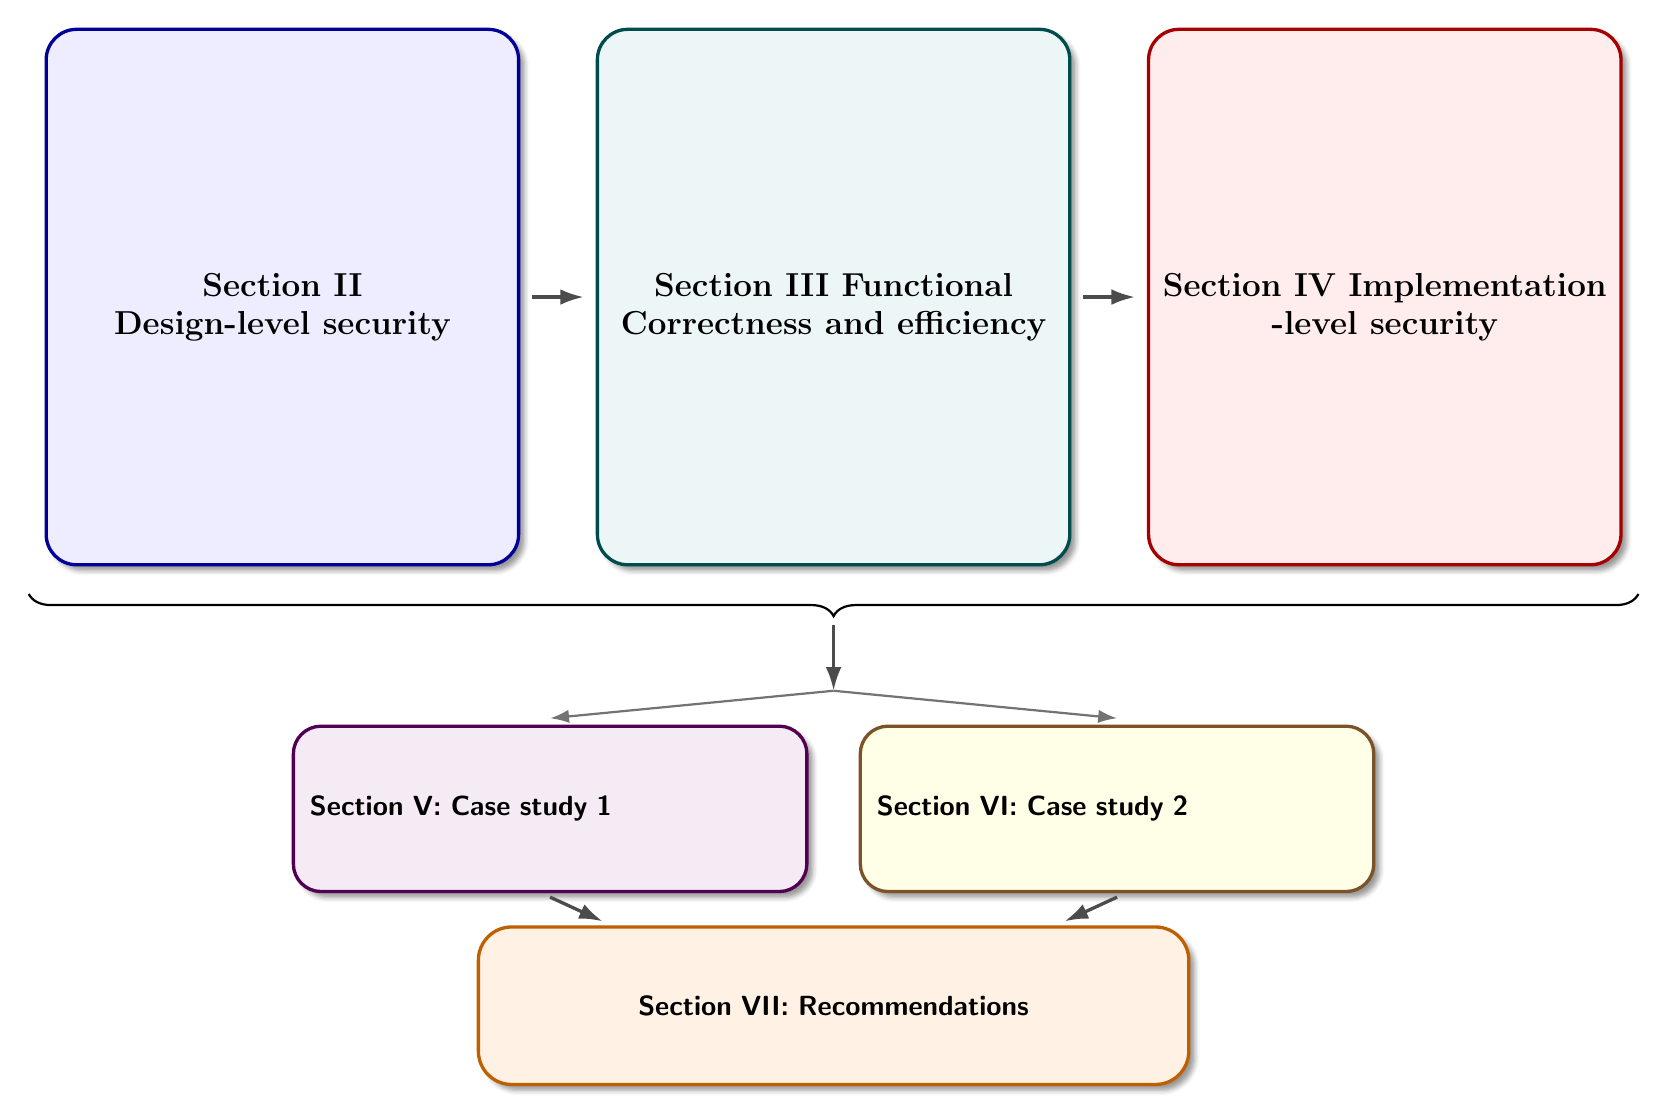
\begin{tikzpicture}[
		font=\sffamily,
		>=Latex,
		title/.style={
			align=center,
			font=\bfseries\Large
		},
		subtitle/.style={
			align=center,
			font=\small,
			text=black!70
		},
		flow/.style={
			-{Latex[length=3mm,width=2mm]},
			very thick,
			draw=black!70
		},
		thinflow/.style={
			-{Latex[length=2.4mm,width=1.7mm]},
			thick,
			draw=black!55
		},
		panelblue/.style={
			draw=blue!60!black,
			very thick,
			rounded corners=11pt,
			fill=blue!7,
			minimum width=6cm,
			minimum height=6.8cm,
			blur shadow={shadow blur steps=4}
		},
		panelgreen/.style={
			draw=teal!60!black,
			very thick,
			rounded corners=11pt,
			fill=teal!7,
			minimum width=6cm,
			minimum height=6.8cm,
			blur shadow={shadow blur steps=4}
		},
		panelred/.style={
			draw=red!65!black,
			very thick,
			rounded corners=11pt,
			fill=red!7,
			minimum width=6cm,
			minimum height=6.8cm,
			blur shadow={shadow blur steps=4}
		},
		innerbox/.style={
			draw=black!55,
			rounded corners=6pt,
			fill=white,
			text width=4.35cm,
			align=left,
			inner sep=4.5pt
		},
		footerbox/.style={
			draw=black!55,
			rounded corners=6pt,
			fill=black!2,
			text width=4.35cm,
			align=center,
			inner sep=4pt
		},
		tag/.style={
			draw=black!45,
			rounded corners=3pt,
			fill=black!3,
			minimum width=4.5mm,
			minimum height=4.2mm,
			inner sep=1pt,
			font=\bfseries\scriptsize
		},
		caseA/.style={
			draw=violet!65!black,
			very thick,
			rounded corners=10pt,
			fill=violet!8,
			text width=6.1cm,
			minimum height=2.1cm,
			align=left,
			inner sep=6pt,
			blur shadow={shadow blur steps=4}
		},
		caseB/.style={
			draw=brown!65!black,
			very thick,
			rounded corners=10pt,
			fill=yellow!10,
			text width=6.1cm,
			minimum height=2.1cm,
			align=left,
			inner sep=6pt,
			blur shadow={shadow blur steps=4}
		},
		finalbox/.style={
			draw=orange!75!black,
			very thick,
			rounded corners=12pt,
			fill=orange!10,
			text width=8.6cm,
			minimum height=2.0cm,
			align=center,
			inner sep=6pt,
			blur shadow={shadow blur steps=4}
		}
		]
		
		% ------------------------------------------------------------------
		% Title
		% ------------------------------------------------------------------
%		\node[title] (maintitle) at (7,5.15)
%		{Structure of the Paper};
		
%		\node[subtitle] at (7,4.45)
%		{Three survey sections with a shared internal logic \;\(\rightarrow\)\;
%			two case studies \;\(\rightarrow\)\; final recommendations};
		
		% ------------------------------------------------------------------
		% Legend for A S T U
		% ------------------------------------------------------------------
%		\node[tag] (A) at (11,5.0) {A};
%		\node[anchor=west,font=\scriptsize] at ($(A.east)+(0.08,0)$) {Accuracy};
%		\node[tag] (S) at (13,5.0) {S};
%		\node[anchor=west,font=\scriptsize] at ($(S.east)+(0.08,0)$) {Scope};
%		\node[tag] (T) at (11,4.5) {T};
%		\node[anchor=west,font=\scriptsize] at ($(T.east)+(0.08,0)$) {Trust};
%		\node[tag] (U) at (13,4.5) {U};
%		\node[anchor=west,font=\scriptsize] at ($(U.east)+(0.08,0)$) {Usability};
		
		% ------------------------------------------------------------------
		% Main three panels: II, III, IV
		% ------------------------------------------------------------------
		\node[panelblue]  (secII)  at (0,0)  {};
		\node[panelgreen] (secIII) at (7,0)  {};
		\node[panelred]   (secIV)  at (14,0) {};
		
		% ----- Section II -----
		\node[align=center,font=\bfseries\large,text width=5cm]
		at ($(secII.north)+(0,-3.55)$)
		{Section II\\ Design-level security};
		
%		\node[innerbox] (ii-review) at ($(secII.center)+(0,1.15)$)
%		{\scriptsize
%			\textbf{Critical review}\\
%			Why design-level guarantees matter; where symbolic/computational
%			methods outside CAC may fail; how CAC helps; caveats; needed background.};
%		
%		\node[innerbox] (ii-tax) at ($(secII.center)+(0,-0.40)$)
%		{\scriptsize
%			\textbf{Tool taxonomy}\\
%			State-of-the-art tools are organized by common criteria:
%			\textbf{accuracy}, \textbf{scope}, \textbf{trust}, and \textbf{usability}.};
%		
%		\node[tag] at ($(ii-tax.south)+(-1.25,0.30)$) {A};
%		\node[tag] at ($(ii-tax.south)+(-0.40,0.30)$) {S};
%		\node[tag] at ($(ii-tax.south)+(0.45,0.30)$)  {T};
%		\node[tag] at ($(ii-tax.south)+(1.30,0.30)$)  {U};
%		
%		\node[footerbox] (ii-synth) at ($(secII.center)+(0,-2.05)$)
%		{\scriptsize
%			\textbf{Synthesis}\\
%			Achievements, takeaways, research challenges, and references for further reading.};
%		
%		\draw[thinflow] (ii-review.south) -- (ii-tax.north);
%		\draw[thinflow] (ii-tax.south) -- (ii-synth.north);
		
		% ----- Section III -----
		\node[align=center,font=\bfseries\large,text width=5.5cm]
		at ($(secIII.north)+(0,-3.55)$)
		{Section III Functional\\ Correctness and efficiency};
		
%		\node[innerbox] (iii-review) at ($(secIII.center)+(0,1.15)$)
%		{\scriptsize
%			\textbf{Critical review}\\
%			Why functional correctness and efficiency matter; limits of non-CAC
%			practice; what CAC contributes; caveats; technical background.};
%		
%		\node[innerbox] (iii-tax) at ($(secIII.center)+(0,-0.40)$)
%		{\scriptsize
%			\textbf{Tool taxonomy}\\
%			Tools are compared again through the same four evaluation lenses,
%			allowing direct cross-section comparison.};
%		
%		\node[tag] at ($(iii-tax.south)+(-1.25,0.30)$) {A};
%		\node[tag] at ($(iii-tax.south)+(-0.40,0.30)$) {S};
%		\node[tag] at ($(iii-tax.south)+(0.45,0.30)$)  {T};
%		\node[tag] at ($(iii-tax.south)+(1.30,0.30)$)  {U};
%		
%		\node[footerbox] (iii-synth) at ($(secIII.center)+(0,-2.05)$)
%		{\scriptsize
%			\textbf{Synthesis}\\
%			Broader lessons, main achievements, important takeaways, challenges,
%			and further reading.};
%		
%		\draw[thinflow] (iii-review.south) -- (iii-tax.north);
%		\draw[thinflow] (iii-tax.south) -- (iii-synth.north);
		
		% ----- Section IV -----
		\node[align=center,font=\bfseries\large,text width=6.25cm]
		at ($(secIV.north)+(0,-3.55)$)
		{Section IV Implementation\\-level security};
		
%		\node[innerbox] (iv-review) at ($(secIV.center)+(0,1.15)$)
%		{\scriptsize
%			\textbf{Critical review}\\
%			Focus on concrete implementation security, especially resistance to
%			digital side-channel attacks; role of CAC; caveats; background.};
%		
%		\node[innerbox] (iv-tax) at ($(secIV.center)+(0,-0.40)$)
%		{\scriptsize
%			\textbf{Tool taxonomy}\\
%			Implementation-level tools are classified using the same
%			\textbf{A/S/T/U} framework for consistency with Sections II and III.};
		
%		\node[tag] at ($(iv-tax.south)+(-1.25,0.30)$) {A};
%		\node[tag] at ($(iv-tax.south)+(-0.40,0.30)$) {S};
%		\node[tag] at ($(iv-tax.south)+(0.45,0.30)$)  {T};
%		\node[tag] at ($(iv-tax.south)+(1.30,0.30)$)  {U};
%		
%		\node[footerbox] (iv-synth) at ($(secIV.center)+(0,-2.05)$)
%		{\scriptsize
%			\textbf{Synthesis}\\
%			Achievements, takeaways, open challenges, and references for
%			deeper study.};
%		
%		\draw[thinflow] (iv-review.south) -- (iv-tax.north);
%		\draw[thinflow] (iv-tax.south) -- (iv-synth.north);
		
		% Arrows between the three core sections
		\draw[flow] ($(secII.east)+(0.15,0)$) -- ($(secIII.west)+(-0.15,0)$);
		\draw[flow] ($(secIII.east)+(0.15,0)$) -- ($(secIV.west)+(-0.15,0)$);
		
		% Brace under II-IV
		\draw[
		decorate,
		decoration={brace,mirror,amplitude=8pt},
		thick
		]
		($(secII.south west)+(-0.20,-0.35)$) --
		($(secIV.south east)+(0.20,-0.35)$)
		node[midway,below=9pt,align=center,font=\bfseries]
		{
%			Core survey arc:\\same internal template, different technical layer
		};
		
		% ------------------------------------------------------------------
		% Case studies V and VI
		% ------------------------------------------------------------------
		\coordinate (hub) at (7,-5);
		
		\node[caseA] (secV) at (3.4,-6.5)
		{\textbf{Section V: Case study 1}\\
%			Combine tools that address different parts of the problem space and
%			consolidate their guarantees.
		};
		
		\node[caseB] (secVI) at (10.6,-6.5)
		{\textbf{Section VI: Case study 2}\\
%			Distill lessons from the computer-aided cryptography community's
%			involvement in the TLS 1.3 standardization effort.
		};
		
		\draw[flow] ($(secIII.south)+(0,-0.75)$) -- ($(hub.north)$);
		\draw[thinflow] (hub) -- ($(secV.north)+(0,0.08)$);
		\draw[thinflow] (hub) -- ($(secVI.north)+(0,0.08)$);
		
%		\node[font=\small\bfseries,align=center] at ($(hub)+(0,0.28)$)
%		{From surveyed methods to worked examples};
		
		% ------------------------------------------------------------------
		% Final recommendations VII
		% ------------------------------------------------------------------
		\node[finalbox] (secVII) at (7,-9)
		{\textbf{Section VII: Recommendations}\\
%			Guidance for \textbf{paper authors}, \textbf{tool developers}, and
%			\textbf{standardization bodies} on how to move computer-aided
%			cryptography forward.
		};
		
		\draw[flow] ($(secV.south)+(0,-0.05)$) -- ($(secVII.north west)+(1.6,0.05)$);
		\draw[flow] ($(secVI.south)+(0,-0.05)$) -- ($(secVII.north east)+(-1.6,0.05)$);
		
		% ------------------------------------------------------------------
		% Background grouping halo
		% ------------------------------------------------------------------
%		\begin{scope}[on background layer]
%			\node[
%			draw=black!20,
%			rounded corners=16pt,
%			line width=0.8pt,
%			fill=black!1,
%			fit=(secII)(secIII)(secIV)(secV)(secVI)(secVII),
%			inner sep=10pt
%			] {};
%		\end{scope}
		
	\end{tikzpicture}
\end{document}